\documentclass[11pt]{article}
\usepackage[utf8]{inputenc}
\usepackage[T1]{fontenc}
\usepackage[spanish]{babel}
\usepackage{times}
\usepackage{anysize}
\usepackage{verbatim}
\usepackage{float}

%%%%%%%%%%%%%%%%%%%%%%%%%%%%%%%%%%% PARA CODIGO %%%%%%%%%%%%%%
\usepackage{color}
\definecolor{gray97}{gray}{.97}
\definecolor{gray75}{gray}{.75}
\definecolor{gray45}{gray}{.45}

\usepackage{listings}
\lstset{ frame=Ltb,
framerule=0pt,
aboveskip=0.5cm,
framextopmargin=3pt,
framexbottommargin=3pt,
framexleftmargin=0.4cm,
framesep=0pt,
rulesep=.4pt,
backgroundcolor=\color{gray97},
rulesepcolor=\color{black},
%
stringstyle=\ttfamily,
showstringspaces = false,
basicstyle=\small\ttfamily,
commentstyle=\color{gray45},
keywordstyle=\bfseries,
%
numbers=left,
numbersep=15pt,
numberstyle=\tiny,
numberfirstline = false,
breaklines=true,
}

% minimizar fragmentado de listados
\lstnewenvironment{listing}[1][]
{\lstset{#1}\pagebreak[0]}{\pagebreak[0]}

\lstdefinestyle{consola}
{basicstyle=\scriptsize\bf\ttfamily,
backgroundcolor=\color{gray75},
}

\lstdefinestyle{C}
{language=C++,
}

\lstdefinestyle{SQL} {language=SQL}


%\begin{lstlisting}[style=C]
%%codigo
%\end{lstlisting} 
%%%%%%%%%%%%%%%%%%%%%%%%%%%%%%%%%%% PARA CODIGO %%%%%%%%%%%%%%

%% Margenes
\marginsize{3cm}{2cm}{2cm}{2cm}

%Portada
\title{\textbf{\huge{Diseño y Desarrollo de Sistemas de Información. Proyecto Final.}}}
\author{Alejandro Trujillo Caballero}
\date{\today}

\usepackage{graphicx}
\begin{document}

\maketitle
\thispagestyle{empty}
\newpage

\tableofcontents
\newpage

\section{Introducción}

En esta práctica se pretende realizar el proceso completo de diseño e implementación de un sistema de información. Partiendo de un enunciado del cual se extraerán los requisitos, se realizará en diagrama entidad-relación del cuál se extraerá el modelo lógico a implementar en el servidor Oracle del laboratorio de práticas mediante SQL. 

Para el manejo de esta base de datos, se implementará una aplicación en Java que se conectará remotamente al servidor.

\section{Diseño de la base de datos.}

\begin{figure}[H]
\centering
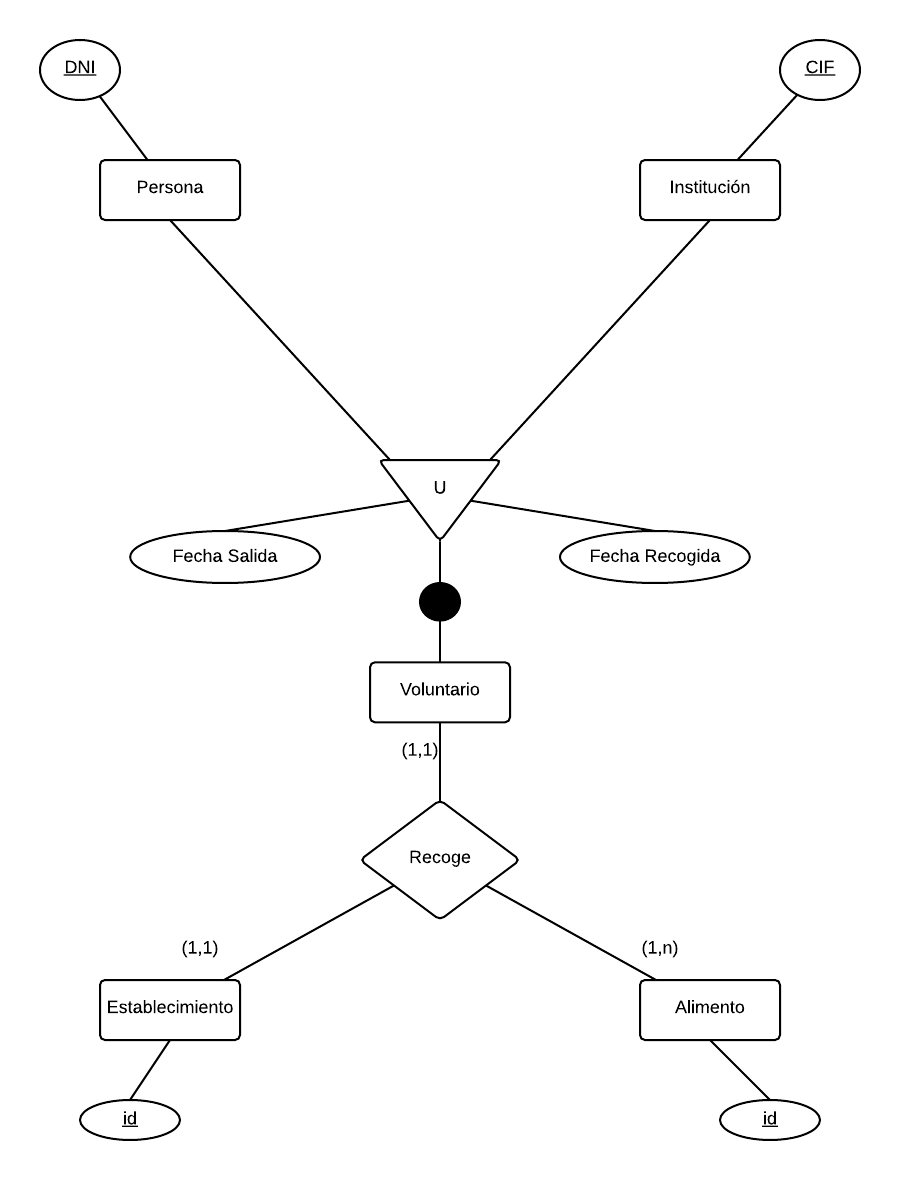
\includegraphics[scale=0.9]{DDSI.png}
\caption{Diagrama Entidad-Relación de la base de datos}
\label{diagrama}
\end{figure}

En la figura \ref{diagrama} se expone el diagrama entidad-relación diseñado para cumplir los requisitos del enunciado. Solo se han incluido los atributos que forman las claves primarias de las entidades de cara a facilitar la comprensión de la estructura general.

Los atributos de cada una de las entidades son:

\paragraph{Persona: }
 DNI, nombre, apellidos, edad, correo electrónico, localidad, teléfono.
 
\paragraph{Institución: }
CIF, nombre, razón social, teléfono.

\paragraph{Establecimiento: }
Id, nombre, dirección, localidad.

\paragraph{Alimento: }
Id, descripción, fecha de caducidad.

\section{Modelo lógico de la base de datos e implementación}

Explicaremos la transformación al modelo lógico de la base de datos directamente sobre el código SQL utilizado para crearla:

\begin{lstlisting}[style=SQL]
--------- TABLA ALIMENTO --------------------------------------
drop table ALIMENTO CASCADE CONSTRAINT;

create table ALIMENTO (
	id number,
	descripcion varchar(50) not null,
	fecha_caducidad date not null,
	
	CONSTRAINT alimentoClave 
		PRIMARY KEY (id)
);
\end{lstlisting}
La entidad Alimento se transforma de forma directa en una tabla que contiene sus atributos y su clave primaria.

\begin{lstlisting}[style=SQL]

-------- TABLA ESTABLECIMIENTO ---------------------------------
drop table ESTABLECIMIENTO CASCADE CONSTRAINT;

create table ESTABLECIMIENTO (
	id number,
	nombre varchar(50) not null,
	direccion varchar(50) not null,
	localidad varchar(50) not null,
	

	CONSTRAINT establecimientoClave 
		PRIMARY KEY (id)
);
\end{lstlisting}
La entidad Establecimiento, al igual que alimento se transforma en una tabla de manera directa.

\begin{lstlisting}[style=SQL]
------- TABLA VOLUNTARIO ---------------------------------------
drop table VOLUNTARIO CASCADE CONSTRAINT;

create table VOLUNTARIO (
	id number,

	CONSTRAINT voluntarioCalve 
		PRIMARY KEY (id)
);
\end{lstlisting}

La categoría Voluntario se traduce como una tabla que unicamente contiene la clave mediante la cual se unificarán Persona e Institución.

\begin{lstlisting}[style=SQL]
-------- TABLA INSTITUCION -------------------------------------
drop table INSTITUCION CASCADE CONSTRAINT;

create table INSTITUCION (
	cif char(9),
	nombre varchar(50) not null,
	razon_social varchar(50),
	telefono number not null,
	idVoluntario number not null UNIQUE,

	CONSTRAINT institucionClave 
		PRIMARY KEY (cif),
	CONSTRAINT voluntarioAjena 
		FOREIGN KEY (idVoluntario) REFERENCES VOLUNTARIO (id) on delete cascade
);
\end{lstlisting}

La entidad Institución se traduce a una tabla, con el atributo añadido idVoluntario como clave ajena a la tabla Voluntario.
\begin{lstlisting}[style=SQL]
------- TABLA PERSONA ------------------------------------------
drop table PERSONA CASCADE CONSTRAINT;

create table PERSONA (
	dni char(9),
	nombre varchar(50) not null,
	apellido1 varchar(50) not null,
	apellido2 varchar(50),
	edad number(2) not null,
	e_mail varchar(50),
	localidad varchar(50) not null,
	telefono number not null,
	idVoluntario number not null UNIQUE,

	CONSTRAINT personaClave 
		PRIMARY KEY (dni),
	CONSTRAINT volAjena 
		FOREIGN KEY (idVoluntario) REFERENCES VOLUNTARIO (id) on delete cascade
);
\end{lstlisting}

La entidad Persona se traduce de forma análoga a Institución.		
\begin{lstlisting}[style=SQL]
------ TABLA RECOGE --------------------------------------------
drop table RECOGE CASCADE CONSTRAINT;

create table RECOGE (
	alimento number,
	voluntario number not null,
	establecimiento number not null,
	fecha_recogida date not null,
	fecha_salida date,
	entregado number(1),

	CONSTRAINT recogeClave 
		PRIMARY KEY (alimento),
	CONSTRAINT alimentoAjena 
		FOREIGN KEY (alimento) REFERENCES ALIMENTO (id),
	CONSTRAINT voluntarioAje
		FOREIGN KEY (voluntario) REFERENCES VOLUNTARIO (id) on delete set null,
	CONSTRAINT establecimientoAjena 
		FOREIGN KEY (establecimiento) REFERENCES ESTABLECIMIENTO (id) on delete set null

);
\end{lstlisting} 
La relación Recoge se traduce como una tabla independiente, con claves ajenas a alimento, voluntario y establecimiento.

El control de la consistencia de las claves de idVoluntario para personas e instituciones se realizará utilizando dos disparadores:

\begin{lstlisting}[style=SQL]
create or replace trigger institucion_o_persona 
	before insert on INSTITUCION
	for each row
	DECLARE
		idVoluntario_erroneo EXCEPTION;
		cantidad number;
	BEGIN
		SELECT count(*) INTO cantidad
		FROM PERSONA p
		WHERE p.idVoluntario = :new.idVoluntario;
		IF cantidad <> 0 THEN
			RAISE idVoluntario_erroneo;
		END IF;	
	END
;
\end{lstlisting} 

\begin{lstlisting}[style=SQL]
create or replace trigger persona_o_institucion
	before insert on PERSONA
	for each row
	DECLARE
		idVoluntario_erroneo EXCEPTION;
		cantidad number;
	BEGIN
		SELECT count(*) INTO cantidad
		FROM INSTITUCION I
		WHERE I.idVoluntario = :new.idVoluntario;
		IF cantidad <> 0 THEN
			RAISE idVoluntario_erroneo;
		END IF;	
	END
;
\end{lstlisting} 

\section{Aplicación Java}
El programa Java será un aplicación de consola que contemplará en un menú las opciones de inserción/consulta/modificación/borrado que se solicitan en el enunciado.

\subsection{Estructura de clases}
El código de la aplicación se divide en los cuatro paquetes que se citan a continuación, se explicará brevemente el contenido de cada uno de ellos pero no se incluirá código en esta memoria debido a su extensión.

\paragraph{Aplicación: }
Contiene la estructura básica de la aplicación, el main y la conexión al servidor.

\paragraph{Consola: }
Contiene la definición del menú de consola y el control de la entrada por teclado.

\paragraph{Datos: }
Contiene las clases que representan a cada una de las tablas y entidades de la base de datos, de cara a trabajar con ellas con facilidad.

\paragraph{Persistencia: }
Contiene las clases que manejan la lógica y la comunicación con la base de datos (inserciones, consultas...).  

\end{document}
